\documentclass[12pt]{article}
\setlength{\oddsidemargin}{0in}
\setlength{\evensidemargin}{0in}
\setlength{\textwidth}{6.5in}
\setlength{\parindent}{0in}
\setlength{\parskip}{\baselineskip}

\usepackage[all]{xy}

\usepackage{amsmath,amsfonts,amssymb}
\usepackage{graphicx}
\usepackage{fancyhdr}
\pagestyle{fancy}
\usepackage{hyperref}

\begin{document}

\lhead{{\bf CSCI 3104 \\ Problem Set 9} }
\rhead{Name: \fbox{Michael Rogers} \\ ID: \fbox{105667404} \\ {\bf Profs.\ Grochow \& Layer\\ Spring 2019, CU-Boulder}}
\renewcommand{\headrulewidth}{0.5pt}
\phantom{Test}

Quick links \ref{1a} \ref{1b} \ref{1c} \ref{1d} \ref{2} \ref{3}


\vspace{-3mm}
\begin{enumerate}

	\item (30 pts) Bidirectional breadth-first search is a variant of standard BFS for finding a shortest path between two vertices $s,t \in V(G)$. The idea is to run \emph{two} breadth-first searches simultaneously, one starting from $s$ and one starting from $t$, and stop when they ``meet in the middle'' (that is, whenever a vertex is encountered by both searches). ``Simultaneously'' here doesn't assume you have multiple processors at your disposal; it's enough to alternate iterations of the searches: one iteration of the loop for the BFS that started at $s$ and one iteration of the loop for the BFS that started at $t$.
	
	As we'll see, although the worst-case running time of BFS and Bidirectional BFS are asymptotically the same, in practice Bidirectional BFS often performs significantly better.
	
	Throughout this problem, all graphs are unweighted, undirected, simple graphs.
	
	\begin{enumerate}
	\item \label{1a} (5 pts) Give examples to show that, in the worst case, the asymptotic running time of bidirectional BFS is the same as that of ordinary BFS. Note that because we are asking for asymptotic running time, you actually need to provide an infinite family of examples $(G_n, s_n, t_n)$ such that $s_n,t_n \in V(G_n)$, the asymptotic running time of BFS and bidirectional BFS are the same on inputs $(G_n, s_n, t_n)$, and $|V(G_n)| \to \infty$ as $n \to \infty$.
	\\ \\ I don't know
	\pagebreak
	
	\item \label{1b} (5 pts) Recall that in ordinary BFS we used a \texttt{visited} array (see Lecture Notes 8) to keep track of which nodes had been visited before. In bidirectional BFS we'll need \emph{two} \texttt{visited} arrays, one for the BFS from $s$ and one for the BFS from $t$. Let ``naive bidirectional BFS'' denote an attempted implementation of bidirectional BFS which uses only one {\tt visited} array.  Give an example to show what can go wrong if there's only one \texttt{visited} array. More specifically, give a graph $G$ and two vertices $s,t$ such that some run of a naive bidirectional BFS says there is no path from $s$ to $t$ when in fact there is one.
	\\ \\ I don't know
	\pagebreak
	
	\item \label{1c} Consider BFS vs. bidirectional BFS on grids. Namely, let $G_n$ be an $n \times n$ grid, where each vertex is connected to its neighbors in the four cardinal directions (N,S,E,W). Vertices on the boundary of the grid will only have 3 neighbors, and corners will only have 2 neighbors. Let $s_n$ be the midpoint of one edge of the grid, and $t_n$ the midpoint of the opposite edge. For example, for $n=3$ we have:
	
	\[
\xymatrix{
\bullet \ar@{-}[r] \ar@{-}[d] & \bullet \ar@{-}[r] \ar@{-}[d] & \bullet \ar@{-}[d] \\ 
s_3 \ar@{-}[r] \ar@{-}[d] & \bullet \ar@{-}[r] \ar@{-}[d] & t_3 \ar@{-}[d] \\ 
\bullet \ar@{-}[r] & \bullet \ar@{-}[r] & \bullet
}
\]

	\begin{enumerate}
	\item (5 pts) Give an argument as to why BFS starting from $s_n$ searches nearly the entire graph (in fact, a constant fraction of it) before encountering $t_n$. 
	\\ \\ I don't know
	\pagebreak
	
	\item (5 pts) Bidirectional BFS also searches a constant fraction of the entire graph before finding a path from $s_n$ to $t_n$, but a smaller constant fraction than ordinary BFS. Estimate this constant, and give an argument to justify your estimate. Hint: as $n \to \infty$, if you ``zoom out'' the graph starts to look more like the unit square $[0,1] \times [0,1]$ in the real plane $\mathbb{R}^2$. Consider the ``spreading'' picture of BFS / bidirectional BFS and use basic geometric facts.  \\ \\
	\end{enumerate}
	I don't know
	\pagebreak
	
	\item \label{1d} Consider BFS vs. bidirectional BFS on trees. Let $T_n$ is a complete binary tree of depth $n$. $s_n$ is the root and $t_n$ is any leaf. For example, for $n=3$ we have:
	\[
	\xymatrix{
 	   & & & s_3 \ar@{-}[lld] \ar@{-}[rrd] \\ 
	  & \bullet \ar@{-}[dr] \ar@{-}[dl] & & & & \bullet \ar@{-}[dr] \ar@{-}[dl] \\
	\bullet & & \bullet & & t_3 & & \bullet
	}
	\]
	
	\begin{enumerate}
	\item (5 pts) Prove the asymptotic running time of BFS on $T_n$ starting at $s_n$, where the BFS can stop as soon as it finds a path from $s_n$ to $t_n$.
	\\ \\ I don't know
	\pagebreak

	\item (5 pts) Prove the asymptotic running time of bidirectional BFS on $T_n$ starting at $(s_n, t_n)$.
	\\ \\ I don't know
	\pagebreak
	
	\end{enumerate}		
	\end{enumerate}
	

	\item \label{2} (10 pts) Let $G=(V,E)$ be a graph with an edge-weight function $w$, and let the tree $T\subseteq E$ be a minimum spanning tree on $G$. Now, suppose that we modify $G$ slightly by decreasing the weight of exactly one of the edges in $(x,y)\in T$ in order to produce a new graph $G'$. Here, you will prove that the original tree $T$ is still a minimum spanning tree for the modified graph $G'$. \\
	 To get started, let $k$ be a positive number and define the weight function $w'$ as
%
\begin{displaymath}
w'(u,v) = \left\{
\begin{array}{ll}
w(u,v) & \textrm{if $(u,v)\not= (x,y)$} \\
w(x,y)-k & \textrm{if $(u,v)=(x,y)$} \enspace .
\end{array}\right.
\end{displaymath}
%
Now, prove that the tree $T$ is a minimum spanning tree for $G'$, whose edge weights are given by $w'$.
	\\ \\ I don't know
	\pagebreak





	\item \label{3} (20 pts) Professor Snape gives you the following unweighted graph and asks you to construct a weight function $w$ on the edges, using positive integer weights only, such that the following conditions are true regarding minimum spanning trees and single-source shortest path trees:
	\begin{itemize}
	\itemsep-0.1pt
	\item The MST is distinct from any of the seven SSSP trees.
	\item The order in which Jarn\'ik/Prim's algorithm adds the safe edges is different from the order in which Kruskal's algorithm adds them.
	\item Bor$\rm{\dot{u}}$vka's algorithm takes at least two rounds to construct the MST.
	\end{itemize}
	Justify your solution by (i) giving the edges weights, (ii) showing the corresponding MST and all the SSSP trees, and (iii) giving the order in which edges are added by each of the three algorithms. (For Bor$\rm{\dot{u}}$vka's algorithm, be sure to denote which edges are added simultaneously in a single round.)

% ----- FIGURE 1 : adjacency_list.eps -----
\begin{figure}[h!]
\begin{center}
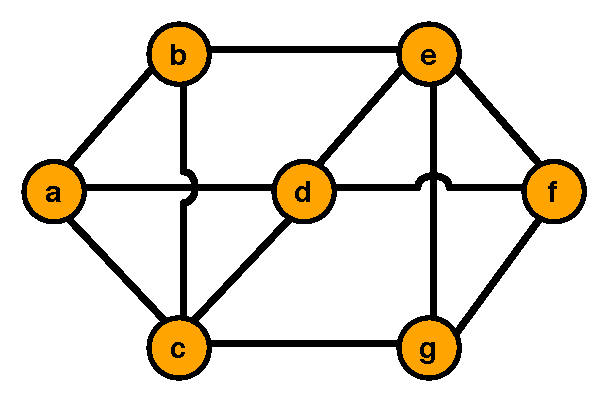
\includegraphics[scale=0.7]{graph_mst.pdf} 
\end{center}
\end{figure}
% ----------

	I don't know


	
	

	
\end{enumerate}


\end{document}

